%%%%%%%%%%%%%%%%%%%%%%%%%%%%%%%%%%%%%%%%%%%%%%%%%%%%%%%%%%%%%%%%%%%%%%%%%%%
%% This file is part of the book
%%
%% Algorithmic Graph Theory
%% http://code.google.com/p/graph-theory-algorithms-book/
%%
%% Copyright (C) 2009, 2010, 2011 Minh Van Nguyen <nguyenminh2@gmail.com>
%%
%% See the file COPYING for copying conditions.
%%%%%%%%%%%%%%%%%%%%%%%%%%%%%%%%%%%%%%%%%%%%%%%%%%%%%%%%%%%%%%%%%%%%%%%%%%%

\subfigure[December~1969]{
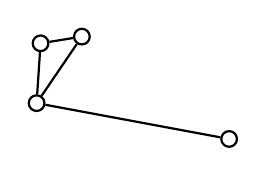
\begin{tikzpicture}
[lineDecorate/.style={-,thick},%
  nodeDecorate/.style={shape=circle,inner sep=2pt,draw,thick},
  scale=0.5]
%% nodes or vertices
\foreach \nodename/\x/\y in {
  0/2.24/6.13, 1/2.34/7.65, 2/3.39/7.82, 3/7.13/5.22}
{
  \node (\nodename) at (\x,\y) [nodeDecorate] {};
}
edges or lines
\path
\foreach \startnode/\endnode in {
  0/1, 0/2, 0/3, 1/2}
{
  (\startnode) edge[lineDecorate] node {} (\endnode)
};
\end{tikzpicture}
}
%%
%%
\qquad
\subfigure[June~1970]{
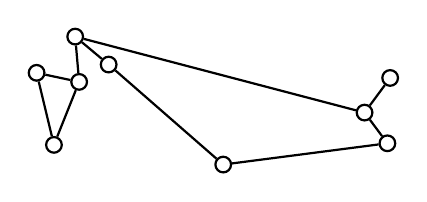
\begin{tikzpicture}
[lineDecorate/.style={-,thick},%
  nodeDecorate/.style={shape=circle,inner sep=2pt,draw,thick},
  scale=0.5]
%% nodes or vertices
\foreach \nodename/\x/\y in {
  0/1.83/7.82, 1/2.27/5.99, 2/2.91/7.59, 3/2.81/8.74, 4/3.66/8.03,
  5/6.57/5.49, 6/10.74/6.03, 7/10.16/6.81, 8/10.81/7.69}
{
  \node (\nodename) at (\x,\y) [nodeDecorate] {};
}
%% edges or lines
\path
\foreach \startnode/\endnode in {
  1/0, 1/2, 2/0, 2/3, 3/4, 4/5, 3/7, 5/6, 7/8, 7/6}
{
  (\startnode) edge[lineDecorate] node {} (\endnode)
};
\end{tikzpicture}
}
%%
%%
\qquad
\subfigure[December~1970]{
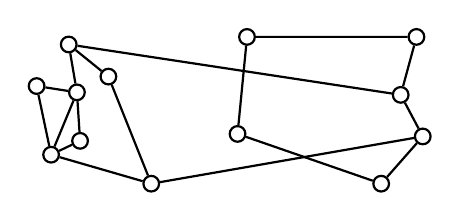
\begin{tikzpicture}
[lineDecorate/.style={-,thick},%
  nodeDecorate/.style={shape=circle,inner sep=2pt,draw,thick},
  scale=0.8]
%% nodes or vertices
\foreach \nodename/\x/\y in {
  0/2.11/5.59, 1/1.60/4.93, 2/2.24/4.83, 3/1.83/3.84, 4/2.29/4.06,
  5/2.74/5.08, 6/3.42/3.38, 7/4.79/4.17, 8/4.94/5.71, 9/7.07/3.38,
  10/7.73/4.13, 11/7.38/4.79, 12/7.63/5.71}
{
  \node (\nodename) at (\x,\y) [nodeDecorate] {};
}
%% edges or lines
\path
\foreach \startnode/\endnode in {
  3/4, 3/1, 3/2, 4/2, 1/2, 2/0, 0/5, 3/6, 5/6, 7/8, 6/10, 7/9, 9/10,
  0/11, 8/12, 11/12, 10/11}
{
  (\startnode) edge[lineDecorate] node {} (\endnode)
};
\end{tikzpicture}
}
%%
%%
\subfigure[September~1971]{
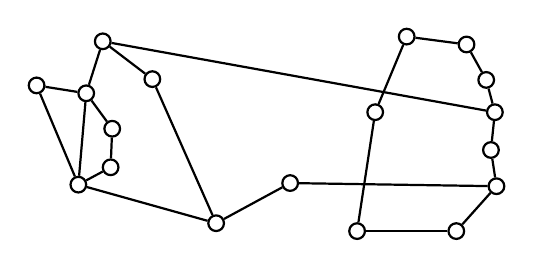
\begin{tikzpicture}
[lineDecorate/.style={-,thick},%
  nodeDecorate/.style={shape=circle,inner sep=2pt,draw,thick},
  scale=1]
%% nodes or vertices
\foreach \nodename/\x/\y in {
  0/2.01/6.27, 1/1.17/5.71, 2/1.80/5.61, 3/2.64/5.79, 4/2.13/5.16,
  5/1.70/4.45, 6/2.11/4.67, 7/3.45/3.96, 8/4.39/4.47, 9/5.47/5.37,
  10/5.24/3.86, 11/5.87/6.33, 12/6.63/6.23, 13/6.88/5.78,
  14/6.99/5.37, 15/6.94/4.89, 16/7.01/4.43, 17/6.50/3.86}
{
  \node (\nodename) at (\x,\y) [nodeDecorate] {};
}
%% edges or lines
\path
\foreach \startnode/\endnode in {
  5/6, 5/2, 5/1, 6/4, 2/1, 2/4, 2/0, 0/3, 5/7, 3/7, 7/8, 0/14, 8/16,
  10/9, 10/17, 17/16, 9/11, 11/12, 12/13, 13/14, 14/15, 15/16}
{
  (\startnode) edge[lineDecorate] node {} (\endnode)
};
\end{tikzpicture}
}
%%
%%
\qquad
\subfigure[March~1972]{
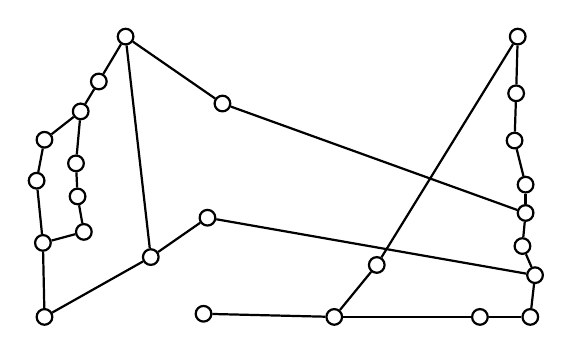
\begin{tikzpicture}
[lineDecorate/.style={-,thick},%
  nodeDecorate/.style={shape=circle,inner sep=2pt,draw,thick},
  scale=1]
%% nodes or vertices
\foreach \nodename/\x/\y in {
  0/2.03/5.21, 1/1.93/4.69, 2/2.01/3.90, 3/2.49/5.57, 4/2.72/5.95,
  5/3.06/6.52, 6/2.43/4.91, 7/2.45/4.49, 8/2.53/4.04, 9/2.03/2.96,
  10/3.38/3.72, 11/4.29/5.67, 12/4.05/3, 13/4.10/4.22,
  14/5.71/2.96, 15/6.25/3.62, 16/7.56/2.96, 17/8.20/2.96,
  18/8.26/3.49, 19/8.10/3.86, 20/8.14/4.28, 21/8.14/4.64,
  22/8/5.2, 23/8.02/5.8, 24/8.04/6.52}
{
  \node (\nodename) at (\x,\y) [nodeDecorate] {};
}
%% edges or lines
\path
\foreach \startnode/\endnode in {
  9/2, 9/10, 2/8, 2/1, 1/0, 7/8, 7/6, 3/0, 4/3, 4/5, 5/11, 5/10,
  10/13, 12/14, 14/15, 14/16, 13/18, 16/17, 11/20, 15/24, 24/23,
  23/22, 22/21, 21/20, 20/19, 19/18, 18/17, 3/6}
{
  (\startnode) edge[lineDecorate] node {} (\endnode)
};
\end{tikzpicture}
}
%%
%%
\subfigure[August~1972]{
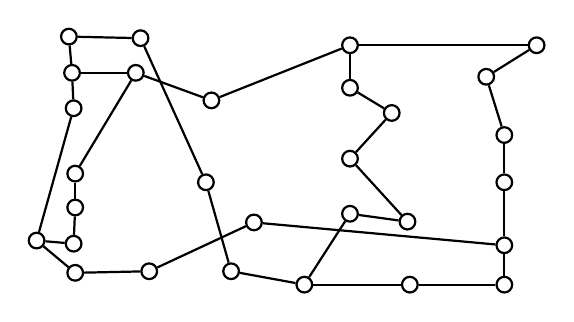
\begin{tikzpicture}
[lineDecorate/.style={-,thick},%
  nodeDecorate/.style={shape=circle,inner sep=2pt,draw,thick},
  scale=1]
%% nodes or vertices
\foreach \nodename/\x/\y in {
  0/1.20/6.85, 1/2.11/6.83, 2/1.24/6.39, 3/2.05/6.39, 4/1.26/5.94,
  5/1.28/5.11, 6/1.28/4.68, 7/0.79/4.26, 8/1.26/4.22, 9/1.28/3.85,
  10/2.22/3.87, 11/2.94/5, 12/3.01/6.04, 13/3.26/3.87,
  14/3.55/4.49, 15/4.19/3.70, 16/4.77/4.6, 17/5.53/3.70,
  18/5.5/4.5, 19/4.77/5.3, 20/5.30/5.88, 21/4.77/6.2,
  22/4.77/6.74, 23/7.14/6.74, 24/6.5/6.34, 25/6.73/5.6,
  26/6.73/5, 27/6.73/4.2, 28/6.73/3.70}
{
  \node (\nodename) at (\x,\y) [nodeDecorate] {};
}
%% edges or lines
\path
\foreach \startnode/\endnode in {
  9/7, 7/8, 7/4, 8/6, 6/5, 5/3, 4/2, 2/3, 2/0, 1/0, 1/11, 10/9, 10/14,
  3/12, 12/22, 11/13, 13/15, 15/17, 17/28, 14/27, 15/16, 16/18, 18/19,
  19/20, 20/21, 21/22, 28/27, 27/26, 26/25, 25/24, 24/23, 23/22}
{
  (\startnode) edge[lineDecorate] node {} (\endnode)
};
\end{tikzpicture}
}
%%
%%
\qquad
\subfigure[September~1973]{
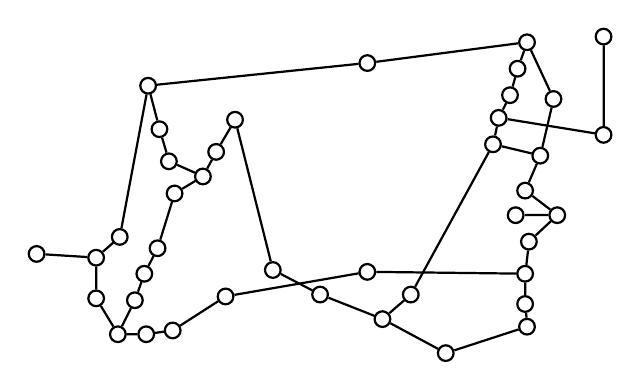
\begin{tikzpicture}
[lineDecorate/.style={-,thick},%
  nodeDecorate/.style={shape=circle,inner sep=2pt,draw,thick},
  scale=1.2]
%% nodes or vertices
\foreach \nodename/\x/\y in {
  0/4.18/5.68, 1/4.30/5.22, 2/4.40/4.88, 3/4.90/4.98, 4/5.10/5.32,
  5/4.76/4.72, 6/4.46/4.54, 7/3.88/4.08, 8/3.63/3.86, 9/3/3.90,
  10/4.28/3.96, 11/4.14/3.69, 12/3.63/3.43, 13/4.04/3.41,
  14/3.86/3.05, 15/4.16/3.05, 16/4.44/3.09, 17/5/3.45,
  18/5.5/3.73, 19/6/3.47, 20/6.5/3.71, 21/6.66/3.21,
  22/6.96/3.47, 23/7.33/2.85, 24/8.19/3.13, 25/8.17/3.37,
  26/8.17/3.69, 27/8.21/4.03, 28/8.51/4.31, 29/8.07/4.31,
  30/8.17/4.57, 31/8.33/4.94, 32/7.83/5.06, 33/7.89/5.34,
  34/8.01/5.58, 35/8.09/5.86, 36/8.19/6.14, 37/6.5/5.92,
  38/8.47/5.54, 39/9/5.16, 40/9/6.20}
{
  \node (\nodename) at (\x,\y) [nodeDecorate] {};
}
%% edges or lines
\path
\foreach \startnode/\endnode in {
  14/15, 15/16, 14/13, 14/12, 12/8, 8/9, 8/7, 13/11, 11/10, 10/6, 6/5,
  7/0, 5/2, 2/1, 1/0, 5/3, 3/4, 0/37, 4/18, 16/17, 17/20, 18/19,
  19/21, 21/23, 21/22, 23/24, 24/25, 25/26, 20/26, 26/27, 27/28,
  28/29, 28/30, 22/32, 30/31, 31/32, 31/38, 32/33, 33/34, 34/35,
  35/36, 36/37, 36/38, 33/39, 39/40}
{
  (\startnode) edge[lineDecorate] node {} (\endnode)
};
\end{tikzpicture}
}
